\documentclass{article}
\usepackage[utf8]{inputenc}
\usepackage{graphicx}
\title{Reporte Tarea 1}
\author{García Lugo Juan}
\date{August 2019}

\begin{document}
\maketitle
\section{Introducción}
En del  este este artículo se encuentra el reporte acerca del desarrollo de la \textsl{''Tarea01''}, la definición del problema, análisis del problema, selección de la mejor alternativa, una explicación del funcionamiento de la aplicación explicado de manera conceptual a través de un diagrama de flujo o pseudocódigo, el mantenimiento y depuración de la aplicación.
\section{Definición del problema}
Se necesita una aplicación que nos muestre en tiempo real tiempo el clima de las ciudades en la base de datos de un aeropuerto donde se estan registrados los vuelos del día, el clima tiene que ser al tiempo al que se ejecute el programa.

La base de datos está definida de la siguiente manera, sea i un renglón de la base de datos con i $>$ 1, i = ciudada de origen, ciudad de destino, latitud origen, longitud origen, latitud destino, longitud destino.
\section{Análisis del problema}
En el problema nos piden una aplicación que nos proporcione el clima en tiempo real , de las ciudades de origen y de llegada, con sus respectivas coordenadas, entonces el flujo general del programa debería de ser el siguiente leer la base de datos, obtener el clima en tiempo real de las ciudades, mostrar el clima de las ciudades de los vuelos en la base de datos, en este caso los   problemas o puntos principales que tendremos que resolver para desarrollar la aplicación son los siguientes.
\begin{itemize}
    \item Leer una base de datos con formato csv: al leer la base de datos tendremos que obtener las ciudades para poder conocer el clima de dicha ciudad.
    \item Obtener el clima en tiempo real: para ello se necesita de un servidor web que cumpla con lo que pedimos.
    \item Evitar saturar el servidor: para eso tendremos que modelar un cache donde se guarden las ciudades que ya han realizado una petición del clima en el web service
\end{itemize}

\section{Selección de la mejor alternativa}
Para realizar este proyecto había varias alternativas que eran bastante buenas, pero en este python ganó ya que es un lenguaje de alto nivel, fácil de aprender , con una sintaxis muy amena, es fácil leer archivos, y tiene una gran variedad de librerías que sirven para la interacción con un web service. 
\section{Diagrama de flujo}
\begin{figure}[h]
    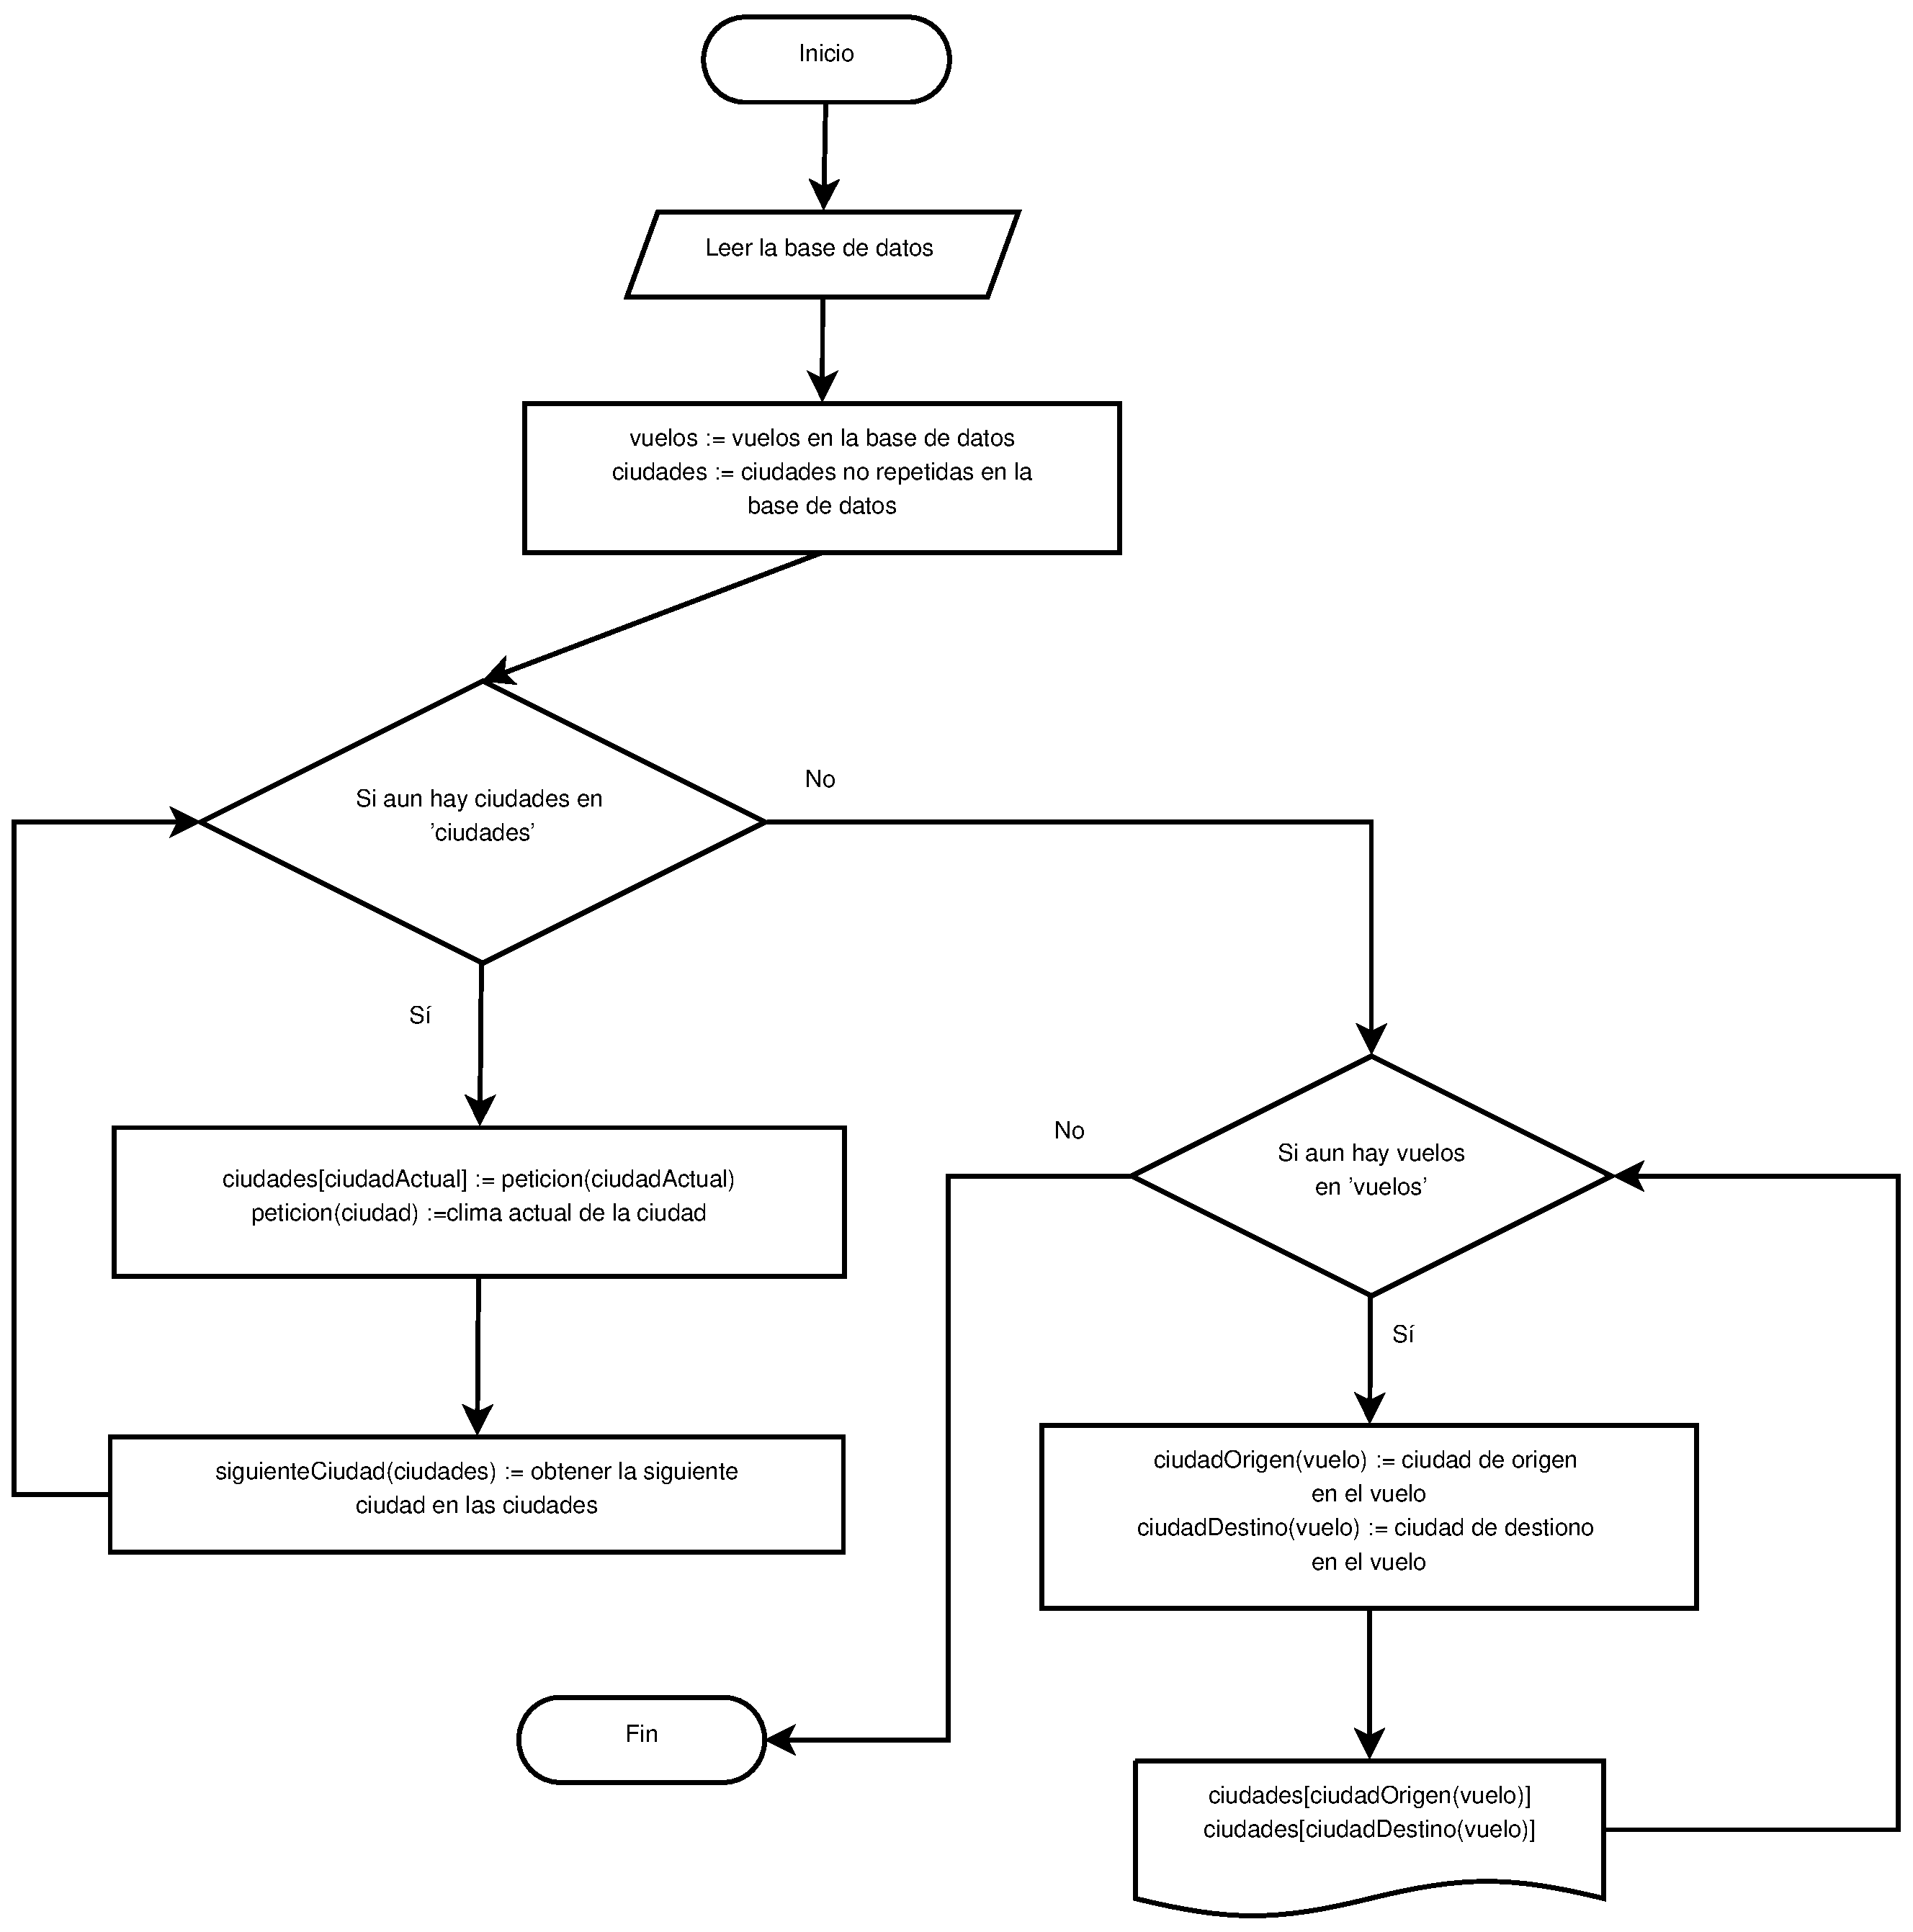
\includegraphics[scale=.26]{imagenes/DiagramaDeFlujo.eps} 
    \caption{Diagrama de Flujo}
    \label{fig:my_label}
\end{figure}
Como podemos notar en la figura 1 el flujo del programa es bastante sencillo, esto se logra por la repartición de deberes en los distintos módulos en python de la aplicación, y librerías utilizadas , pero vamos a describirlo.
\newline
\newline
El flujo del programa del programa se describe de manera secuencial, pero no se describen todas rutinas que realiza el programa ya que la función del diagrama es sólo para mostrar en general que es lo que realiza el 
programa 
\begin{itemize}
    \item Se lee la base de datos.
    \item Se guardan los vuelos de la base de datos.
    \item A partir de los vuelos en la base de datos se obtiene un diccionario con todas las ciudades donde las llaves del diccionario son las ciudades.
    \item Se iteran las llaves del diccionario y con las mismas se realiza una petición a la web service, y el valor de cada llave será el resultado de la petición.
    \item Por último se iteran los vuelos guardados, que contienen las ciudades de origen y de llegada, ambas ciudades se ocupan como llaves para obtener el clima de dicha ciudad.
\end{itemize}
\section{Mantenimiento y costo del software}
Ahora que nuestro programa cumple con los requisitos funcionales, lo mejor sería implementar requisitos no funcionales tales como: una interfaz gráfica que permita al usuario añadir su base de datos a través de una ventana, manejar hilos de ejecución, para poder realizar las peticiones más rápido, y tener un mecanismo que actualice el clima de las ciudades cada cierto tiempo, suponiendo que se llegase a dar el mantenimiento mencionado, creo que un buen precio por el software sería de 10,000 con mantenimiento de un año  
\end{document}
